\documentclass[11pt,a4paper]{article}
\usepackage{fontspec}
\usepackage{babel}
\babelprovide[import,main]{english}
\babelfont{rm}{Noto Serif}
\babelfont{sf}{Noto Sans}
\babelfont{tt}{DejaVu Sans Mono}
\usepackage[a4paper,margin=23mm,headheight=14pt,headsep=8mm]{geometry}
\usepackage{amsmath,amssymb,amsthm,mathtools,stmaryrd}
\usepackage{booktabs,tabularx,array,enumitem,microtype,xcolor,fancyhdr,hyperref,tikz}
\usetikzlibrary{arrows.meta,positioning}
\definecolor{ink}{RGB}{29,53,80}
\definecolor{muted}{RGB}{92,100,110}
\hypersetup{colorlinks=true,linkcolor=ink,citecolor=ink,urlcolor=ink,
  pdftitle={Hypothesis Languages and Proof-Carrying Representation Escalation},
  pdfauthor={Aleksandr Strand}}
\setlength{\parindent}{0pt}
\setlength{\parskip}{5pt plus 1.3pt minus .7pt}
\setlength{\emergencystretch}{3em}
\setlist[enumerate]{leftmargin=1.7em,topsep=3pt,itemsep=2pt}
\setlist[itemize]{leftmargin=1.7em,topsep=3pt,itemsep=2pt}
\pagestyle{fancy}\fancyhf{}
\fancyhead[L]{\footnotesize\color{muted}Hypothesis Languages and Representation Escalation}
\fancyhead[R]{\footnotesize\color{muted}A. Strand}
\fancyfoot[C]{\footnotesize\color{muted}\thepage}
\renewcommand{\headrulewidth}{.3pt}
\newtheorem{definition}{Definition}[section]
\newtheorem{theorem}{Theorem}[section]
\newtheorem{proposition}{Proposition}[section]
\newtheorem{remark}{Remark}[section]
\newcommand{\F}{\mathbb{F}}
\newcommand{\sem}[1]{\llbracket #1\rrbracket}
\newcommand{\VS}{\widetilde V}
\newcommand{\Agree}{\operatorname{Agree}}
\newcommand{\Bs}{\operatorname{Bs}}
\newcommand{\DFA}{\operatorname{DFA}}
\newcommand{\oneDCA}{\operatorname{1\text{-}DCA}}
\newcommand{\vstatus}[1]{\textsf{#1}}
\title{\bfseries\color{ink}Hypothesis Languages and Proof-Carrying Representation Escalation\\[4pt]
\large\normalfont From Finite Impossibility Certificates to Parametric Theorems for Counter and Stack Automata}
\author{Aleksandr Strand}
\date{23 November 2026}
\begin{document}
\maketitle
\vspace{-1.0em}
\begin{abstract}
We treat the choice of a hypothesis language as an explicit condition on identification and on justified representational change. For semantic version spaces, we establish monotonicity under additional observations, the potential loss of uniqueness under language enlargement, and an exact identification window for linear Boolean hypothesis families. For finite-state machines, a matrix of distinguishing prefixes and suffixes gives a finite certificate that an unknown target function cannot be implemented by a DFA subject to a specified state bound; it does not establish the nonregularity of an arbitrary black box. The stronger Gate~12 result connects bounded automatic synthesis of a two-phase stack automaton to a parametric Lean~4 theorem: when a candidate program $P$ satisfies the decidable canonical-structure predicate and a binary map $f$ distinguishes the two bits, its specification holds over all $\Sigma^*$ and it is separated from \emph{every} finite-control DFA and one-counter machine in the \emph{declared formal models}. Two instances, $u\#u^R$ and $u\#\overline u^R$, use the same checker. Validating the ordering of selected exported observation prefixes does not prove the absence of lookahead in the actual Python controller's oracle-call history. We distinguish formal theorems, finite tests, and assumptions about the authenticity of an external oracle.
\end{abstract}

\section{Semantic identification and language change}

We describe a claimed invariant by $\mathcal I=\langle\Phi,\mathcal D,\mathcal T,\mathcal E\rangle$: its assertion, scope and assumptions, class of transformations, and type of checkable evidence. Such a record does not in itself increase the claim's evidential status.

\begin{definition}[Semantic version space]
Let $Q$ be the set of admissible queries, $A$ the set of responses, $\mathcal L$ a program language, $\sem\cdot:\mathcal L\to A^Q$ its interpretation, and $D\subseteq Q\times A$ a finite observation set. Define
\begin{equation}\label{eq:version}
\VS(\mathcal L,D)=\{\sem h:h\in\mathcal L,\ \forall(q,a)\in D\ \sem h(q)=a\}\subseteq A^Q.
\end{equation}
Programs with identical behavior over the entire declared $Q$ represent one semantic hypothesis, even if their source programs differ.
\end{definition}

With fixed semantics, additional consistent observations can only shrink the version space. A semantics-preserving language embedding can only enlarge it:
\begin{equation}\label{eq:monotonic}
\begin{aligned}
D\subseteq D'&\Longrightarrow\VS(\mathcal L,D')\subseteq\VS(\mathcal L,D),\\
\mathcal L_i\hookrightarrow\mathcal L_j&\Longrightarrow\VS(\mathcal L_i,D)\subseteq\VS(\mathcal L_j,D).
\end{aligned}
\end{equation}
Consequently, $|\VS(\mathcal L_i,D)|=1$ need not persist in a richer $\mathcal L_j$. The label $\vstatus{IDENTIFIED}$ is always relative to a language and semantic domain.

Two different identification demands exchange the order of quantifiers:
\begin{align}\label{eq:quantifiers}
&\forall i\ \forall f^\star\in\sem{\mathcal L_i}\ \exists D_i\text{ finite}:\quad
 \VS(\mathcal L_i,D_i)=\{f^\star\};\\
&\exists D\text{ finite}\ \forall i\ (f^\star\in\sem{\mathcal L_i})\Rightarrow
 \VS(\mathcal L_i,D)=\{f^\star\}.
\end{align}
Neither statement is \emph{postulated} for an arbitrary infinite hierarchy. The first may hold for each finite bounded language without implying the second, which demands a common $D$.

For example, on $Q=\F_2^2$ the answers $f(0,0)=0$ and $f(1,0)=1$ uniquely identify $f=x_1$ among functions depending only on $x_1$, but leave \emph{four} total Boolean functions when all $f:Q\to\F_2$ are admitted. The number of syntax trees need not equal the number of distinct behaviors on $Q$.

\section{The two-sided identification window in linear Boolean languages}

Let $Q=\F_2^n$ and $R=\F_2[x_1,\ldots,x_n]/(x_1^2-x_1,\ldots,x_n^2-x_n)$ be the algebra of Boolean functions represented by multilinear polynomials. Consider nested finite-dimensional linear spaces $U_0\subseteq\cdots\subseteq U_m\subseteq R$, the observation support $Z\subseteq Q$, and consistent labels $y\in\F_2^Z$.

Write $\rho_Z:U_i\to\F_2^Z$ for the restriction map and $K_i=\ker(\rho_Z|_{U_i})=U_i\cap I(Z)$, where $I(Z)$ is the ideal of functions vanishing on $Z$.

\begin{theorem}[Identification window]\label{thm:window}
If $\rho_Z(f)=y$ is solvable in $U_i$, its solution space is the affine coset $f_i+K_i$, and
\begin{equation}\label{eq:affine}
|\VS(U_i,D)|=2^{\dim U_i-\operatorname{rank}(\rho_Z|_{U_i})}.
\end{equation}
Let $i_*(D)$ be the first level admitting a solution and $k_{\rm break}(Z)$ the first level with $K_i\ne\{0\}$; use $+\infty$ if the relevant level does not exist. Then
\begin{equation}\label{eq:window}
|\VS(U_i,D)|=1\quad\Longleftrightarrow\quad i_*(D)\le i<k_{\rm break}(Z).
\end{equation}
\end{theorem}
\begin{proof}
When the equation is solvable, the inverse image of $y$ under the linear restriction map is a translate of its kernel. Nesting makes solvability monotone in $i$ and the kernels nested. Exactly one solution exists after the first solvable level and before the first nonzero kernel.
\end{proof}

For a nonempty affine version space, a query $q\in Q\setminus Z$ divides the remaining functions evenly between $0$ and $1$ \emph{if and only if} evaluation $p\mapsto p(q)$ is a nonzero linear functional on $K_i$. This exact bisection property of the linear case cannot be extended to arbitrary grammars without additional assumptions.

\section{Distinguishing hypotheses and testing a model}

\begin{definition}[Agreement set]
For a \emph{nonempty} set $V\subseteq A^Q$, define
\begin{equation}\label{eq:agree}
\Agree(V)=\{q\in Q:\forall f,g\in V\ \ f(q)=g(q)\}.
\end{equation}
\end{definition}

At $q\notin\Agree(V)$ surviving hypotheses predict different outcomes, so the experiment can distinguish candidates. At $q\in\Agree(V)$ all predict one response: a different, trustworthy and admissible response makes $\VS(\mathcal L,D\cup\{(q,a)\})=\varnothing$, refuting the \emph{current language and its assumptions}. For $|A|>2$ even a disagreement query may return an outcome no candidate predicts.

\begin{figure}[htbp]
\centering
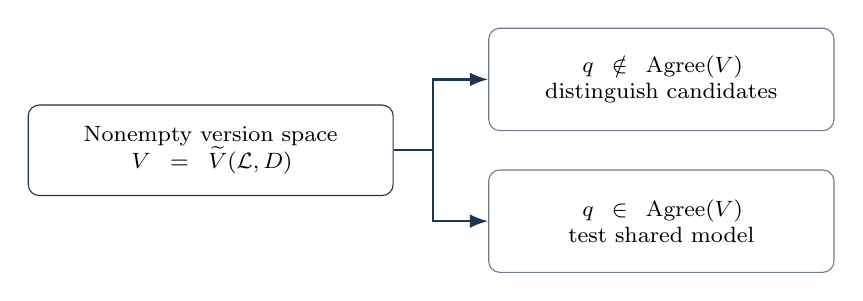
\begin{tikzpicture}[>=Latex,font=\footnotesize,node distance=6mm]
\node[draw=ink,rounded corners,align=center,text width=4.4cm,minimum height=1.15cm] (v) {Nonempty version space\\$V=\VS(\mathcal L,D)$};
\node[draw=ink!65,rounded corners,align=center,text width=4.15cm,minimum height=1.30cm,right=1.2cm of v,yshift=9mm] (d) {$q\notin\Agree(V)$\\distinguish candidates};
\node[draw=ink!65,rounded corners,align=center,text width=4.15cm,minimum height=1.30cm,right=1.2cm of v,yshift=-9mm] (f) {$q\in\Agree(V)$\\test shared model};
\draw[->,thick,ink] (v.east) -- ++(5mm,0) |- (d.west);
\draw[->,thick,ink] (v.east) -- ++(5mm,0) |- (f.west);
\end{tikzpicture}
\caption{One query interface supports two logically different experimental purposes. A unique surviving hypothesis is not by itself a test of the language's applicability.}\label{fig:query}
\end{figure}

When $V=\varnothing$, the universal quantification in~\eqref{eq:agree} holds vacuously; it must not be interpreted as successful agreement. Inconsistency might indicate model misspecification, damaged measurements, or an incorrect association of the observational context. The fact $|V|=0$ does not by itself identify the cause.

\subsection{Language expansion as a checkable action}

For transformations $T_i:\mathcal L\mapsto\mathcal L_i$, define the predicted answer sets given data $D$:
\begin{equation}\label{eq:cross}
P_i(q\mid D)=\{f(q):f\in\VS(\mathcal L_i,D)\}.
\end{equation}
If $P_i(q\mid D)$ and $P_j(q\mid D)$ are nonempty and disjoint, a trustworthy answer $a$ at $q$ eliminates at least one competing language. This tests \emph{ways of extending a representation}, not just individual programs. The order of two transformations may matter: $T_i(T_j(\mathcal L))$ need not equal $T_j(T_i(\mathcal L))$. Actual noncommutativity requires an exhibited witness; it does not follow merely from naming two operators.

When it exists, the minimal inconsistent prefix is
\begin{equation}\label{eq:failprefix}
t_{\rm fail}(\mathcal L)=\min\{t:\VS(\mathcal L,D_{\le t})=\varnothing\}.
\end{equation}
A certificate must establish nonemptiness on the preceding prefix and absence of candidates on this one; finite enumeration or a sound UNSAT proof must identify the exact grammar version. The more expressive language is not thereby established as true merely because the smaller one was refuted.

\section{A finite local construction with a Rule 110 base layer}

The cellular experiment uses a periodic ring of $64$ cells. Its base binary layer follows Rule~110 up to the internal write-back, while cell roles, phases, messages, and registers form an \emph{augmented} local alphabet. Therefore this is not an implementation of the complete observer protocol solely with the two-state Rule~110 alphabet.

For four specifically fixed histories with two contexts, the complete base configurations of each pair coincide at times $10\ldots27$ while auxiliary memory retains the distinction. Parity is available at state $t=13$, the observation receipt at $t=19$, and the historical bit is written back into the base layer in the transition $27\to28$. The full \emph{augmented} states never merge; determinism is not violated.

Valid observation triples $C_3=\{000,010,110,111\}$ are augmented by $p=z_1\oplus z_A\oplus z_B$:
\begin{equation}\label{eq:code}
C_4=\{0000,0101,1100,1111\},\qquad d_{\min}(C_4)=2.
\end{equation}
This code detects any \emph{single-bit inversion} of a correctly formed word but does not guarantee detection of coordinated two-bit corruption: $10$ of the $24$ two-bit changes produce another valid word. A zero syndrome does not certify the origin of an arbitrary initial 64-bit configuration.

\begin{equation}\label{eq:live}
\begin{aligned}
\mathrm{Cert}_{\rm live}(V,a,z_1,z_A,z_B,p)\ \Longleftrightarrow\quad
 &[V=2^a]\\[-2pt]
 &\land[(z_1,z_A,z_B)\in C_3]\\[-2pt]
 &\land[h_{\rm code}(z_1,z_A,z_B)=a]\\[-2pt]
 &\land[z_1\oplus z_A\oplus z_B\oplus p=0].
\end{aligned}
\end{equation}

Unlike a once-stored flag~\cite{leucker2009}, this predicate refers to \emph{current} register values. It does not authenticate an arbitrary coordinated overwrite of all fields. The $\vstatus{ORIGIN\_MEMBERSHIP}$ status for an arbitrary origin remains $\vstatus{UNKNOWN}$.

\begin{table}[htbp]
\centering\small
\caption{Scope of formal and computational results for the finite cellular construction}\label{tab:lean}
\renewcommand{\arraystretch}{1.10}
\begin{tabularx}{\linewidth}{@{}>{\raggedright\arraybackslash}p{3.2cm}>{\raggedright\arraybackslash}X>{\raggedright\arraybackslash}p{2.6cm}@{}}
\toprule
\textbf{Group} & \textbf{Checked subject} & \textbf{Evidence}\\
\midrule
Local properties & Algebraic Rule 110 identity, $C_4$ code, finite predicate $\mathrm{Cert}_{\rm live}$ & 10 Lean theorems\\
64-cell bridge & Base layer, merger of four histories, clocks and six register interventions & 5 Lean theorems\\
Observed states & Formal alphabet size, finite traces and selected fault classes & Experimental record\\
\bottomrule
\end{tabularx}
\end{table}

The supplied Lean~4.36.0 logs record successful completion of both modules without \texttt{sorry}. The five spacetime theorems list the standard \texttt{propext} axiom; they apply to the \emph{four} enumerated histories and their specified finite times. They do not establish soundness for all $2^{64}$ initial configurations or unbounded time. The previous edition reports $23\,014\,938\,240$ formal field configurations per cell and $505$ observed local states on nominal traces. The former counts a Cartesian product of declared fields; the latter is finite-run data, not a minimal-state theorem.

Any memory lower bound must also state its scope: if one accessible context must distinguish \emph{five pairwise distinct} outcomes, at least five internal states are necessary. Merging \emph{two} histories in each fixed context does not alone establish such a five-state lower bound for the whole construction.

\section{Finite escalation of a Boolean hypothesis language}

A separate Python prototype~\cite{jha2017}, \texttt{gate6\_autonomous\_escalation.py}, uses $Q=\F_2^3$ (eight inputs) and a predefined hierarchy of algebraic normal form languages of degrees $\le1,\le2,\le3$. The controller selects distinguishing queries, tests an apparently unique survivor on previously unseen points and escalates after $|\VS(\mathcal L_i,D)|=0$.

The five built-in tests pass: targets $x_1x_2$, $x_1x_2x_3$, and $x_1\oplus x_3$ trigger one, two, and zero escalations, respectively. Disabling escalation blocks a false certificate; modifying stored parity or inserting a false refutation record causes the local checker to reject. This is a \emph{finite} example of degree selection in a predefined grammar, not the invention of an unrestricted new language.

The checker recomputes the version space from current observations and verifies that there are no models for the \emph{present} refutation entries. However, that ledger is a mutable Python list, not a cryptographically immutable audit log; XOR of stored answers does not independently authenticate their truth. Checking all eight inputs before accepting does not establish transfer to an infinite domain.

\section{Gate 11: a finite witness of global impossibility for bounded DFAs}

Here a stronger kind of negative certificate appears. Its domain is the \emph{infinite} set of words $Q=\Sigma^*$, but the excluded model class has a \emph{fixed finite resource bound}.

Let $\Sigma=\{0,1\}$, $k\ge1$, and $f:\Sigma^*\to\{0,1\}$ be a target membership function (or an accurate oracle). By the Myhill--Nerode criterion~\cite{myhill1957,nerode1958}, take prefixes $p_i=0^i$ and suffixes $s_j=1^j$ for $0\le i,j\le k$. Their observed answers form the finite matrix
\begin{equation}\label{eq:mn_matrix}
M_k(i,j)=f(p_is_j)=f(0^i1^j),\qquad 0\le i,j\le k.
\end{equation}
\begin{theorem}[Finite certificate excluding all DFAs with at most $k$ states]\label{thm:bounded_dfa}
If all $(k+1)^2$ verified answers satisfy
\begin{equation}\label{eq:mn_diagonal}
M_k(i,j)=\begin{cases}1,&i=j,\\0,&i\ne j,\end{cases}
\end{equation}
then \emph{no} DFA with $\le k$ states computes $f$ on the entire $\Sigma^*$.
\end{theorem}
\begin{proof}
Suppose such a DFA existed. The $k+1$ prefixes $p_0,\ldots,p_k$ must take it to two equal states after some distinct $p_i$ and $p_j$. Reading the same suffix $s_i=1^i$ would then produce equal acceptance results. Yet~\eqref{eq:mn_diagonal} requires $f(p_is_i)=1$ and $f(p_js_i)=0$. This is a contradiction.
\end{proof}

Although the certificate contains only finitely many answers, it excludes a candidate DFA \emph{as an implementation on all words}: equal internal DFA states would force equal outcomes for any common continuation. The critical premise is that the entries are the \emph{true} answers for the same fixed target $f$, with context and query identities preserved.

\begin{figure}[htbp]
\centering
\begin{tabular}{c|cccc}
$M_3$ & $s_0$ & $s_1$ & $s_2$ & $s_3$\\ \hline
$p_0$ & $\mathbf 1$ & 0 & 0 & 0\\
$p_1$ & 0 & $\mathbf 1$ & 0 & 0\\
$p_2$ & 0 & 0 & $\mathbf 1$ & 0\\
$p_3$ & 0 & 0 & 0 & $\mathbf 1$
\end{tabular}
\caption{Illustration for $k=3$: sixteen answers rule out every DFA with at most three states, not every larger DFA.}\label{fig:matrix}
\end{figure}

\begin{remark}[Limit of a finite oracle]\label{rem:oracle}
For every \emph{fixed} $k$, matrix~\eqref{eq:mn_diagonal} rules out only $\DFA(\le k)$. Without extra assumptions, \emph{no} finite list of queries rules out every finite DFA for an arbitrary unknown target. A regular language can agree with all the finite observations. Thus this experiment alone does not demonstrate nonregularity of the unknown black box.
\end{remark}

For the \emph{formally specified} language
\begin{equation}\label{eq:anbn}
L_{=}=\{0^n1^n:n\ge0\}
\end{equation}
there is a separate kind of result. The public file \href{https://github.com/Dnarts/proof-carrying-discovery/blob/main/formal/DFAto1DCASeparation.lean}{\texttt{DFAto1DCASeparation.lean}} contains \texttt{anbn\_not\_dfa} for \emph{every} $S\in\mathbb N$ and \texttt{anbn1DCA\_accepts} for an explicit deterministic one-counter automaton with three control states. Its Lean~4.36.0 log gives exit code $0$ and standard axiom dependencies \texttt{propext}, \texttt{Classical.choice}, and \texttt{Quot.sound}, as applicable. The quantifier $\forall S$ follows from a \emph{mathematical argument for a defined function}, not a finite sample from an unknown oracle.

An unrelated Python automaton fitted to a finite dataset is not thereby verified for all words. A formally checked semantic connection between the concrete implementation and the Lean definition would be needed.

\section{Gate 12: parametric certification after changing computational memory}

\subsection{The formal family of replacement programs}

Let $\Sigma=\{0,1,\#\}$ and $W=\Sigma^*$. Given a binary transformation $f:\{0,1\}\to\{0,1\}$, define
\begin{equation}\label{eq:mid-language}
L_f=\{u\,\#\,(f(u))^R:\ u\in\{0,1\}^*\},
\end{equation}
where $f(u)$ maps each symbol of $u$ through $f$. The \texttt{StackProgram 2} representation has two control phases: before the separator it pushes the $f$-image of every input bit; after the separator it compares each incoming bit with and removes the top stack symbol. Acceptance requires a valid separator and an empty stack. Nothing here asserts that every DPDA follows this structure.

The decidable predicate \texttt{isCanonicalMidDPDA P f} checks the transitions for every binary symbol and possible stack top, prohibition of repeated separators, admissibility of $f$, and the acceptance condition. The extra condition $f(0)\ne f(1)$ asserts injectivity on the binary alphabet. In that case, only two binary maps remain, identity and bit swap, even if the formal type is $\mathrm{Sym}\to\mathrm{Sym}$.

\begin{theorem}[Parametric specification of a stack automaton]\label{thm:dpda}
For $P:\texttt{StackProgram 2}$ and a binary map $f$ satisfying\
\[\texttt{isCanonicalMidDPDA}(P,f)=\mathrm{true},\]\
the following holds for every $w\in W$:
\begin{equation}\label{eq:dpda-sound}
P.\operatorname{eval}(w)=\mathrm{true}
\quad\Longleftrightarrow\quad
\exists u\in\{0,1\}^*:\ w=u\,\#\,(f(u))^R.
\end{equation}
\end{theorem}
This universal consequence is derived from a parametric inductive proof in {\ttfamily gate12\_\allowbreak hierarchy\_\allowbreak checker.lean}. Checking a concrete exported program's premises using \texttt{by decide} is an \emph{application} of that theorem; it is not replacing induction with finite testing.

\begin{theorem}[Class separation when the binary distinction is preserved]\label{thm:separation}
Under the premises of Theorem~\ref{thm:dpda} and $f(0)\ne f(1)$,
\begin{equation}\label{eq:global-sep}
\begin{aligned}
&\forall k\in\mathbb N:\ \nexists M:\DFA(k),\quad
  \forall w\in W\; M(w)=P(w),\\
&\forall m\in\mathbb N:\ \nexists C:\oneDCA(m),\quad
  \forall w\in W\; C(w)=P(w).
\end{aligned}
\end{equation}
The classes $\DFA(k)$ and $\oneDCA(m)$ refer to the \texttt{DFA} and \texttt{CounterProgram} types in the formal module, not to arbitrary external machine definitions.
\end{theorem}

\begin{proof}[Outline of the second assertion]
Fix $m$ and let $L=2m+2$. There are $2^L$ pairwise distinct binary prefixes of this length. In the formal one-counter model a machine has at most $\operatorname{dcaConfigBound}(m,L)=1+m(L+1)$ configurations after reading such a prefix, including rejection. The Lean arithmetic lemma establishes
\begin{equation}\label{eq:dca-bound}
1+\operatorname{dcaConfigBound}(m,2m+2)\le 2^{2m+2}.
\end{equation}
By pigeonhole, two different binary prefixes reach the same configuration. For injective $f$, the continuation $\#(f(u))^R$ appropriate to one prefix $u$ must be accepted after it and rejected after the other. This contradicts equality of the configurations. For DFA, the usual distinguishing-suffix argument applies.
\end{proof}

If $f(0)=f(1)$, the argument based on distinguishing suffixes no longer applies: language~\eqref{eq:mid-language} depends on $|u|$ and need not retain the individual bits of $u$ in a stack. An explicit converse one-counter construction is \emph{not} among the presented universal Lean theorems; no fully formal two-way classification by this condition is claimed here.

\subsection{Two exported programs and their proofs}

A single controller, \texttt{gate12\_blind\_chomsky\_escalation.py}, found two distinct candidates in a limited grammar and generated one Lean file instantiating the shared theorem. The first uses $f=\mathrm{id}$, the second the involution $f(0)=1$, $f(1)=0$. In both cases the conclusion covers \emph{all} finite words by~\eqref{eq:dpda-sound}, not just a finite experimental horizon. These are two instances of one structural family, \emph{not} evidence of autonomous discovery of every possible DPDA language.

\begin{table}[htbp]
\centering\small
\caption{Executed Gate 12 v12.3 protocol: oracle calls and exported evidence}\label{tab:gate12}
\renewcommand{\arraystretch}{1.15}
\begin{tabularx}{\linewidth}{@{}>{\raggedright\arraybackslash}Xrrr@{}}
\toprule
\textbf{Task} & \textbf{Oracle calls} & \textbf{Recorded} & \textbf{$(t_1,t_2)$}\\
\midrule
$u\#u^R$ & 88 & 60 & $(9,54)$\\
$u\#\overline{u}^R$ & 107 & 61 & $(9,54)$\\
\bottomrule
\end{tabularx}
\end{table}

All three built-in Python tests pass. An independent finite audit tested $29\,524$ words of length at most nine \emph{per task}, with no mismatches, and checked byte-identical regeneration of the exported Lean file. These finite tests do not prove the mathematical theorem over infinite $W$ or the authenticity of the external oracle; the former comes from the formal proof and the latter remains an assumption.

\subsection{Precise boundary of the causal certificate}

The Boolean checker \texttt{checkCausalEscalation} uses a selected observation list $D$ and indices $t_1<t_2$. It checks the inadequacy of $\DFA(k)$ on $D_{\le t_1}$, that of $\oneDCA(m)$ on $D_{\le t_2}$, and agreement of the exported program with all $D$. Together with the canonical predicate, the theorem \texttt{checkFullChomskyProtocol\_sound} yields seven consequences: index ordering, two bounded exclusions, consistency, the infinite specification, and two global class exclusions.

However, $D$ is a \emph{selected exported list}, not the full chronological trace of Python oracle calls. By the time the second witness was completed, $82$ and $100$ oracle queries had actually been made, although $t_2=54$ in both exported lists. Therefore the formal check establishes the \emph{logical sufficiency of selected witness prefixes}, not absence of access to later answers when the controller decided to escalate. The policy state, all oracle requests, and actual response times are not coupled in Lean to the complete execution trace.

Formal verification thus refers to the \emph{exported machine} and its stated premises. It does not constitute a general proof of the Python synthesizer, Python-to-Lean translation, or experimental source authenticity. The sequence DFA$\to$1-DCA$\to$DPDA is a \emph{hierarchy of machine memory}, not three separate levels of the classical Chomsky hierarchy.

\section{Evidence types and proof status}

\begin{table}[htbp]
\centering\small
\caption{Different certification objects over an infinite domain}\label{tab:status}
\renewcommand{\arraystretch}{1.12}
\begin{tabularx}{\linewidth}{@{}>{\raggedright\arraybackslash}p{2.55cm}>{\raggedright\arraybackslash}X>{\raggedright\arraybackslash}p{3.05cm}@{}}
\toprule
\textbf{Status} & \textbf{What is established} & \textbf{Not entailed}\\
\midrule
Class excluded & No DFA with $\le k$ states agrees with the full target $f$ given a trustworthy matrix & Oracle nonregularity\\
Consistent with $D$ & Program explains finite observations & Global correctness\\
Identified within $G$ & One semantic candidate in the fixed $G$ & Uniqueness after changing $G$\\
Formal separation & Given $L_=$ lies outside DFA and has a 1-DCA implementation & All Python programs are correct\\
Canonical DPDA family $L_f$ & Universal specification and separation from $\DFA(k)$, $\oneDCA(m)$ for injective binary $f$ & All DPDAs or real oracle-call history\\
\bottomrule
\end{tabularx}
\end{table}

Semantic identity is not source-code identity. Agreement of observational behavior is not identity of physical causes. A historical receipt does not guarantee integrity of the current register; a parity check does not establish the origin of its observations. These boundaries can become part of a verification protocol, but are not eliminated by relabeling its statuses.

Gate~11 uses a finite matrix to exclude a \emph{resource-bounded class}. Gate~12 adds an independent positive object: global correctness of a \emph{synthesized formal program} once the premises of a parametric theorem have been verified. This does not remove the need to establish actual observation order or oracle fidelity. Both mechanisms rely on established automata and identification theory; the case study's methodological contribution is the combined presentation of its claim, scope, checkable witness, and limits of transfer.

\section{Conclusion}

Semantic identification requires a specified hypothesis language, observation domain, and behavioral equivalence criterion. A finite distinguishing matrix can exclude all machines with a declared resource bound without proving that an arbitrary unknown language is nonregular. For the formal program synthesized in Gate~12, a stronger kind of claim is established: membership in a bounded canonical family gives a checkable route to a universal specification and class separation over the infinite collection of finite words.

This construction demonstrates \emph{proof-carrying} synthesis within a predeclared grammar and a preestablished parametric checker; it does not demonstrate autonomous generation of an unrestricted scientific language. The positive theorem, negative certificates, oracle relativity, and the controller's actual causal history remain distinct justification objects. Maintaining these distinctions is necessary before transferring the method beyond the two fixed binary tasks.

\begin{thebibliography}{99}\setlength{\itemsep}{1pt}
\bibitem{myhill1957} J.~Myhill. \emph{Finite Automata and the Representation of Events}. WADC Technical Report 57--624, 1957.
\bibitem{nerode1958} A.~Nerode. \emph{Linear Automaton Transformations}. Proceedings of the American Mathematical Society, 9(4):541--544, 1958.
\bibitem{moore1956} E.~F.~Moore. \emph{Gedanken-experiments on Sequential Machines}. Automata Studies, pp.~129--153, 1956.
\bibitem{gold1978} E.~M.~Gold. \emph{Complexity of Automaton Identification from Given Data}. Information and Control, 37(3):302--320, 1978.
\bibitem{jha2017} S.~Jha, S.~A.~Seshia. \emph{A Theory of Formal Synthesis via Inductive Learning}. Acta Informatica, 54:693--726, 2017.
\bibitem{hamming1950} R.~W.~Hamming. \emph{Error Detecting and Error Correcting Codes}. Bell System Technical Journal, 29(2):147--160, 1950.
\bibitem{leucker2009} M.~Leucker, C.~Schallhart. \emph{A Brief Account of Runtime Verification}. Journal of Logic and Algebraic Programming, 78(5):293--303, 2009.
\bibitem{gate12code} A.~Strand. \emph{Gate 12 v12.3: parametric two-phase stack certification and class separation}. Lean 4.36.0 source and audit logs, 2026.
\end{thebibliography}
\end{document}
